\begin{figure}[h!]
	\centering
	
	
	% Gradient Info
	
	\tikzset {_jupf8dp9u/.code = {\pgfsetadditionalshadetransform{ \pgftransformshift{\pgfpoint{0 bp } { 0 bp }  }  \pgftransformrotate{0 }  \pgftransformscale{2 }  }}}
	\pgfdeclarehorizontalshading{_oxikznzed}{150bp}{rgb(0bp)=(0.82,0.01,0.11);
		rgb(37.5bp)=(0.82,0.01,0.11);
		rgb(43.973214285714285bp)=(0.97,0.91,0.11);
		rgb(49.24107142857143bp)=(0.72,0.91,0.53);
		rgb(55.58035714285714bp)=(0.11,0.97,0.94);
		rgb(62.00892857142857bp)=(0.8,0.29,0.89);
		rgb(100bp)=(0.8,0.29,0.89)}
	
	% Gradient Info
	
	\tikzset {_rrrrdzg1t/.code = {\pgfsetadditionalshadetransform{ \pgftransformshift{\pgfpoint{0 bp } { 0 bp }  }  \pgftransformrotate{0 }  \pgftransformscale{2 }  }}}
	\pgfdeclarehorizontalshading{_f2np8rf0m}{150bp}{rgb(0bp)=(0.82,0.01,0.11);
		rgb(37.5bp)=(0.82,0.01,0.11);
		rgb(43.973214285714285bp)=(0.97,0.91,0.11);
		rgb(49.24107142857143bp)=(0.72,0.91,0.53);
		rgb(55.58035714285714bp)=(0.11,0.97,0.94);
		rgb(62.00892857142857bp)=(0.8,0.29,0.89);
		rgb(100bp)=(0.8,0.29,0.89)}
	\tikzset{every picture/.style={line width=0.75pt}} %set default line width to 0.75pt        
	
	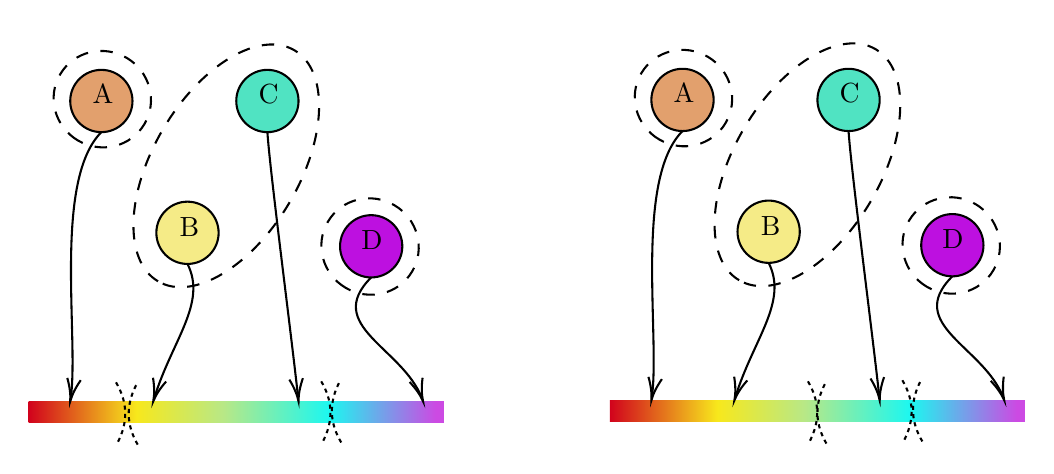
\begin{tikzpicture}[x=0.75pt,y=0.75pt,yscale=-1,xscale=1]
		%uncomment if require: \path (0,300); %set diagram left start at 0, and has height of 300
		
		%Shape: Circle [id:dp8686502462251218] 
		\draw  [fill={rgb, 255:red, 226; green, 160; blue, 109 }  ,fill opacity=1 ] (70,64.97) .. controls (70,56.68) and (76.72,49.97) .. (85,49.97) .. controls (93.28,49.97) and (100,56.68) .. (100,64.97) .. controls (100,73.25) and (93.28,79.97) .. (85,79.97) .. controls (76.72,79.97) and (70,73.25) .. (70,64.97) -- cycle ;
		%Shape: Circle [id:dp5552463587832126] 
		\draw  [fill={rgb, 255:red, 80; green, 227; blue, 194 }  ,fill opacity=1 ] (150,64.97) .. controls (150,56.68) and (156.72,49.97) .. (165,49.97) .. controls (173.28,49.97) and (180,56.68) .. (180,64.97) .. controls (180,73.25) and (173.28,79.97) .. (165,79.97) .. controls (156.72,79.97) and (150,73.25) .. (150,64.97) -- cycle ;
		%Shape: Circle [id:dp21656446486952063] 
		\draw  [fill={rgb, 255:red, 245; green, 235; blue, 135 }  ,fill opacity=1 ] (111.5,128.47) .. controls (111.5,120.18) and (118.22,113.47) .. (126.5,113.47) .. controls (134.78,113.47) and (141.5,120.18) .. (141.5,128.47) .. controls (141.5,136.75) and (134.78,143.47) .. (126.5,143.47) .. controls (118.22,143.47) and (111.5,136.75) .. (111.5,128.47) -- cycle ;
		%Shape: Circle [id:dp6549202348048928] 
		\draw  [fill={rgb, 255:red, 189; green, 16; blue, 224 }  ,fill opacity=1 ] (200,134.97) .. controls (200,126.68) and (206.72,119.97) .. (215,119.97) .. controls (223.28,119.97) and (230,126.68) .. (230,134.97) .. controls (230,143.25) and (223.28,149.97) .. (215,149.97) .. controls (206.72,149.97) and (200,143.25) .. (200,134.97) -- cycle ;
		%Shape: Ellipse [id:dp6213542116896975] 
		\draw  [dash pattern={on 4.5pt off 4.5pt}] (112.3,151.84) .. controls (95.55,141.95) and (96.7,109.01) .. (114.86,78.28) .. controls (133.02,47.55) and (161.32,30.66) .. (178.06,40.55) .. controls (194.81,50.45) and (193.66,83.38) .. (175.5,114.12) .. controls (157.34,144.85) and (129.05,161.74) .. (112.3,151.84) -- cycle ;
		%Shape: Ellipse [id:dp18690290078640293] 
		\draw  [dash pattern={on 4.5pt off 4.5pt}] (73.7,83.97) .. controls (62.49,77.35) and (58.66,63.07) .. (65.16,52.09) .. controls (71.65,41.1) and (86,37.56) .. (97.21,44.19) .. controls (108.42,50.81) and (112.25,65.09) .. (105.75,76.08) .. controls (99.26,87.06) and (84.91,90.6) .. (73.7,83.97) -- cycle ;
		%Shape: Ellipse [id:dp10224302620382786] 
		\draw  [dash pattern={on 4.5pt off 4.5pt}] (202.7,154.97) .. controls (191.49,148.35) and (187.66,134.07) .. (194.16,123.09) .. controls (200.65,112.1) and (215,108.56) .. (226.21,115.19) .. controls (237.42,121.81) and (241.25,136.09) .. (234.75,147.08) .. controls (228.26,158.06) and (213.91,161.6) .. (202.7,154.97) -- cycle ;
		%Shape: Rectangle [id:dp3411009771047675] 
		\draw  [draw opacity=0][shading=_oxikznzed,_jupf8dp9u] (50,220) -- (50,209.97) -- (250,209.97) -- (250,220) -- cycle ;
		%Curve Lines [id:da09977618835584368] 
		\draw    (85,79.97) .. controls (61.73,103.25) and (74.23,178.62) .. (70.27,207.98) ;
		\draw [shift={(70,209.72)}, rotate = 279.63] [color={rgb, 255:red, 0; green, 0; blue, 0 }  ][line width=0.75]    (10.93,-3.29) .. controls (6.95,-1.4) and (3.31,-0.3) .. (0,0) .. controls (3.31,0.3) and (6.95,1.4) .. (10.93,3.29)   ;
		%Curve Lines [id:da6318930308826853] 
		\draw    (215,149.97) .. controls (191.73,173.25) and (230.16,183.8) .. (239.47,208.21) ;
		\draw [shift={(240,209.72)}, rotate = 252.07] [color={rgb, 255:red, 0; green, 0; blue, 0 }  ][line width=0.75]    (10.93,-3.29) .. controls (6.95,-1.4) and (3.31,-0.3) .. (0,0) .. controls (3.31,0.3) and (6.95,1.4) .. (10.93,3.29)   ;
		%Curve Lines [id:da09627170903749671] 
		\draw    (126.5,143.47) .. controls (136.06,162.34) and (118.96,180.48) .. (110.51,208.02) ;
		\draw [shift={(110,209.72)}, rotate = 286.14] [color={rgb, 255:red, 0; green, 0; blue, 0 }  ][line width=0.75]    (10.93,-3.29) .. controls (6.95,-1.4) and (3.31,-0.3) .. (0,0) .. controls (3.31,0.3) and (6.95,1.4) .. (10.93,3.29)   ;
		%Curve Lines [id:da7334611428136537] 
		\draw    (165,79.97) .. controls (166.23,98.84) and (176.34,176.05) .. (179.8,207.83) ;
		\draw [shift={(180,209.72)}, rotate = 263.92] [color={rgb, 255:red, 0; green, 0; blue, 0 }  ][line width=0.75]    (10.93,-3.29) .. controls (6.95,-1.4) and (3.31,-0.3) .. (0,0) .. controls (3.31,0.3) and (6.95,1.4) .. (10.93,3.29)   ;
		%Shape: Boxed Bezier Curve [id:dp6591612969439882] 
		\draw  [dash pattern={on 1.5pt off 1.5pt}]  (102.5,230.5) .. controls (97.25,221.5) and (96.25,211.5) .. (102.5,200.5) ;
		%Shape: Boxed Bezier Curve [id:dp22021352768956315] 
		\draw  [dash pattern={on 1.5pt off 1.5pt}]  (92.05,200.52) .. controls (97.38,209.47) and (98.46,219.47) .. (92.31,230.52) ;
		%Shape: Boxed Bezier Curve [id:dp17420743375708936] 
		\draw  [dash pattern={on 1.5pt off 1.5pt}]  (190.93,200.04) .. controls (196.25,208.99) and (197.34,218.98) .. (191.18,230.04) ;
		%Shape: Boxed Bezier Curve [id:dp21373559969089517] 
		\draw  [dash pattern={on 1.5pt off 1.5pt}]  (200.57,229.49) .. controls (195.2,220.56) and (194.07,210.57) .. (200.18,199.49) ;
		%Shape: Circle [id:dp2071167052111076] 
		\draw  [fill={rgb, 255:red, 226; green, 160; blue, 109 }  ,fill opacity=1 ] (350,64.45) .. controls (350,56.17) and (356.71,49.45) .. (365,49.45) .. controls (373.28,49.45) and (380,56.17) .. (380,64.45) .. controls (380,72.73) and (373.28,79.45) .. (365,79.45) .. controls (356.71,79.45) and (350,72.73) .. (350,64.45) -- cycle ;
		%Shape: Circle [id:dp5086147230828475] 
		\draw  [fill={rgb, 255:red, 80; green, 227; blue, 194 }  ,fill opacity=1 ] (430,64.45) .. controls (430,56.17) and (436.71,49.45) .. (445,49.45) .. controls (453.28,49.45) and (460,56.17) .. (460,64.45) .. controls (460,72.73) and (453.28,79.45) .. (445,79.45) .. controls (436.71,79.45) and (430,72.73) .. (430,64.45) -- cycle ;
		%Shape: Circle [id:dp1132042015881487] 
		\draw  [fill={rgb, 255:red, 245; green, 235; blue, 135 }  ,fill opacity=1 ] (391.5,127.95) .. controls (391.5,119.67) and (398.21,112.95) .. (406.5,112.95) .. controls (414.78,112.95) and (421.5,119.67) .. (421.5,127.95) .. controls (421.5,136.23) and (414.78,142.95) .. (406.5,142.95) .. controls (398.21,142.95) and (391.5,136.23) .. (391.5,127.95) -- cycle ;
		%Shape: Circle [id:dp5225952989546916] 
		\draw  [fill={rgb, 255:red, 189; green, 16; blue, 224 }  ,fill opacity=1 ] (480,134.45) .. controls (480,126.17) and (486.71,119.45) .. (495,119.45) .. controls (503.28,119.45) and (510,126.17) .. (510,134.45) .. controls (510,142.73) and (503.28,149.45) .. (495,149.45) .. controls (486.71,149.45) and (480,142.73) .. (480,134.45) -- cycle ;
		%Shape: Ellipse [id:dp008210969696711645] 
		\draw  [dash pattern={on 4.5pt off 4.5pt}] (392.29,151.33) .. controls (375.55,141.43) and (376.69,108.49) .. (394.85,77.76) .. controls (413.02,47.03) and (441.31,30.14) .. (458.06,40.03) .. controls (474.81,49.93) and (473.66,82.87) .. (455.5,113.6) .. controls (437.34,144.33) and (409.04,161.22) .. (392.29,151.33) -- cycle ;
		%Shape: Ellipse [id:dp15440925630698055] 
		\draw  [dash pattern={on 4.5pt off 4.5pt}] (353.7,83.45) .. controls (342.49,76.83) and (338.66,62.55) .. (345.15,51.57) .. controls (351.64,40.58) and (365.99,37.05) .. (377.21,43.67) .. controls (388.42,50.3) and (392.24,64.57) .. (385.75,75.56) .. controls (379.26,86.54) and (364.91,90.08) .. (353.7,83.45) -- cycle ;
		%Shape: Ellipse [id:dp5043296278196521] 
		\draw  [dash pattern={on 4.5pt off 4.5pt}] (482.7,154.45) .. controls (471.49,147.83) and (467.66,133.55) .. (474.15,122.57) .. controls (480.64,111.58) and (494.99,108.05) .. (506.21,114.67) .. controls (517.42,121.3) and (521.24,135.57) .. (514.75,146.56) .. controls (508.26,157.54) and (493.91,161.08) .. (482.7,154.45) -- cycle ;
		%Shape: Rectangle [id:dp7051919783039517] 
		\draw  [draw opacity=0][shading=_f2np8rf0m,_rrrrdzg1t] (330,219.48) -- (330,209.45) -- (530,209.45) -- (530,219.48) -- cycle ;
		%Curve Lines [id:da37843887018525946] 
		\draw    (365,79.45) .. controls (341.72,102.73) and (354.22,178.11) .. (350.26,207.46) ;
		\draw [shift={(350,209.2)}, rotate = 279.63] [color={rgb, 255:red, 0; green, 0; blue, 0 }  ][line width=0.75]    (10.93,-3.29) .. controls (6.95,-1.4) and (3.31,-0.3) .. (0,0) .. controls (3.31,0.3) and (6.95,1.4) .. (10.93,3.29)   ;
		%Curve Lines [id:da9854017683047185] 
		\draw    (495,149.45) .. controls (471.72,172.73) and (510.16,183.28) .. (519.47,207.69) ;
		\draw [shift={(520,209.2)}, rotate = 252.07] [color={rgb, 255:red, 0; green, 0; blue, 0 }  ][line width=0.75]    (10.93,-3.29) .. controls (6.95,-1.4) and (3.31,-0.3) .. (0,0) .. controls (3.31,0.3) and (6.95,1.4) .. (10.93,3.29)   ;
		%Curve Lines [id:da13498803888212696] 
		\draw    (406.5,142.95) .. controls (416.05,161.82) and (398.96,179.96) .. (390.51,207.51) ;
		\draw [shift={(390,209.2)}, rotate = 286.14] [color={rgb, 255:red, 0; green, 0; blue, 0 }  ][line width=0.75]    (10.93,-3.29) .. controls (6.95,-1.4) and (3.31,-0.3) .. (0,0) .. controls (3.31,0.3) and (6.95,1.4) .. (10.93,3.29)   ;
		%Curve Lines [id:da046756128412226206] 
		\draw    (445,79.45) .. controls (446.22,98.32) and (456.33,175.53) .. (459.8,207.32) ;
		\draw [shift={(460,209.2)}, rotate = 263.92] [color={rgb, 255:red, 0; green, 0; blue, 0 }  ][line width=0.75]    (10.93,-3.29) .. controls (6.95,-1.4) and (3.31,-0.3) .. (0,0) .. controls (3.31,0.3) and (6.95,1.4) .. (10.93,3.29)   ;
		%Shape: Boxed Bezier Curve [id:dp7139533309729651] 
		\draw  [dash pattern={on 1.5pt off 1.5pt}]  (434.32,230) .. controls (429.07,221) and (428.07,211) .. (434.32,200) ;
		%Shape: Boxed Bezier Curve [id:dp4178108981730697] 
		\draw  [dash pattern={on 1.5pt off 1.5pt}]  (425.43,200.04) .. controls (430.75,208.99) and (431.84,218.98) .. (425.68,230.04) ;
		%Shape: Boxed Bezier Curve [id:dp8000489551931103] 
		\draw  [dash pattern={on 1.5pt off 1.5pt}]  (470.92,199.52) .. controls (476.25,208.48) and (477.33,218.47) .. (471.18,229.52) ;
		%Shape: Boxed Bezier Curve [id:dp738862646285132] 
		\draw  [dash pattern={on 1.5pt off 1.5pt}]  (480.56,228.97) .. controls (475.2,220.04) and (474.07,210.05) .. (480.18,198.97) ;
		
		% Text Node
		\draw (79.25,55.47) node [anchor=north west][inner sep=0.75pt]   [align=left] {A};
		% Text Node
		\draw (121.25,119.47) node [anchor=north west][inner sep=0.75pt]   [align=left] {B};
		% Text Node
		\draw (159.25,55.47) node [anchor=north west][inner sep=0.75pt]   [align=left] {C};
		% Text Node
		\draw (208.75,125.97) node [anchor=north west][inner sep=0.75pt]   [align=left] {D};
		% Text Node
		\draw (359.25,54.95) node [anchor=north west][inner sep=0.75pt]   [align=left] {A};
		% Text Node
		\draw (401.25,118.95) node [anchor=north west][inner sep=0.75pt]   [align=left] {B};
		% Text Node
		\draw (439.25,54.95) node [anchor=north west][inner sep=0.75pt]   [align=left] {C};
		% Text Node
		\draw (488.75,125.45) node [anchor=north west][inner sep=0.75pt]   [align=left] {D};
		
		
	\end{tikzpicture}
\end{figure}